%!TEX root = ../main.tex
\subsection{Board Layout} % (fold)
\label{sub:board_layout}
The layout of the board involved a number of considerations, especially concerning the layout of the power part of the circuit.
These considerations involve the layer stack, the required copper thickness and various placements of components.
This section will discuss in appropriate detail these considerations.
Figure \ref{fig:board_layout} is an overview of the final layout of board.
Firstly, it is desirable to determine what requirements exist for the trace widths and thicknesses in the layout.

\begin{figure}
	\begin{subfigure}[b]{\textwidth}
	\centering
	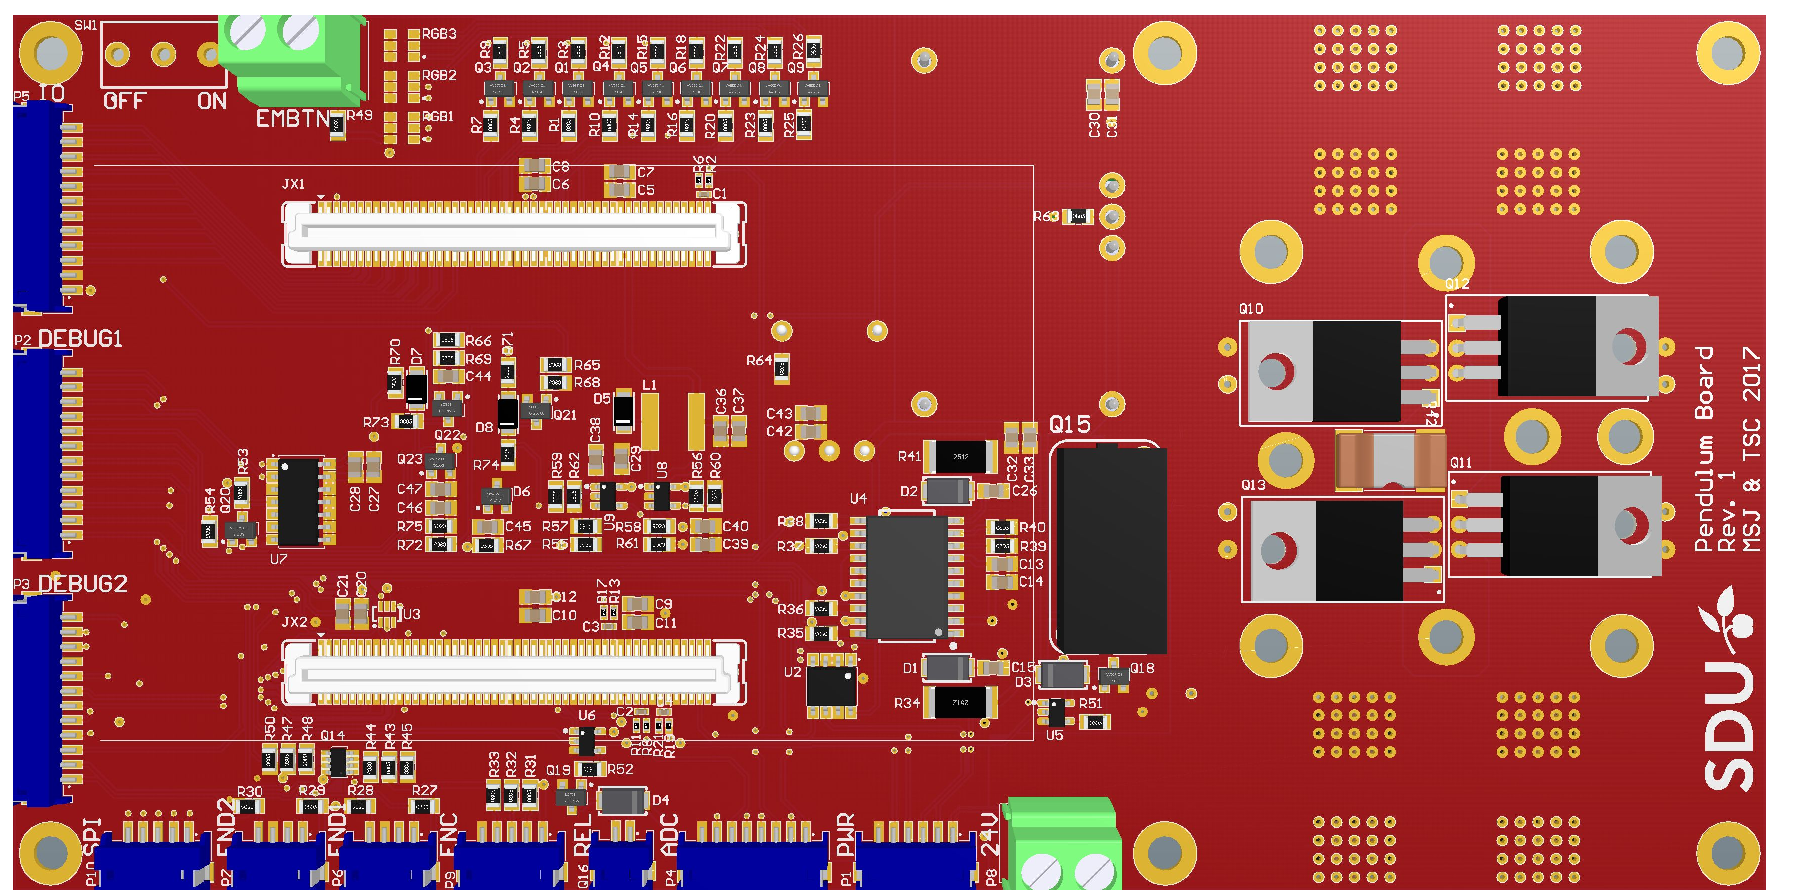
\includegraphics[width=0.8\textwidth]{graphics/top_side_pcb}
	\caption{Top side PCB view of controller board.}
	\label{fig:top_side_pcb_view}
	\end{subfigure}\\

	\begin{subfigure}[b]{\textwidth}
	\centering
	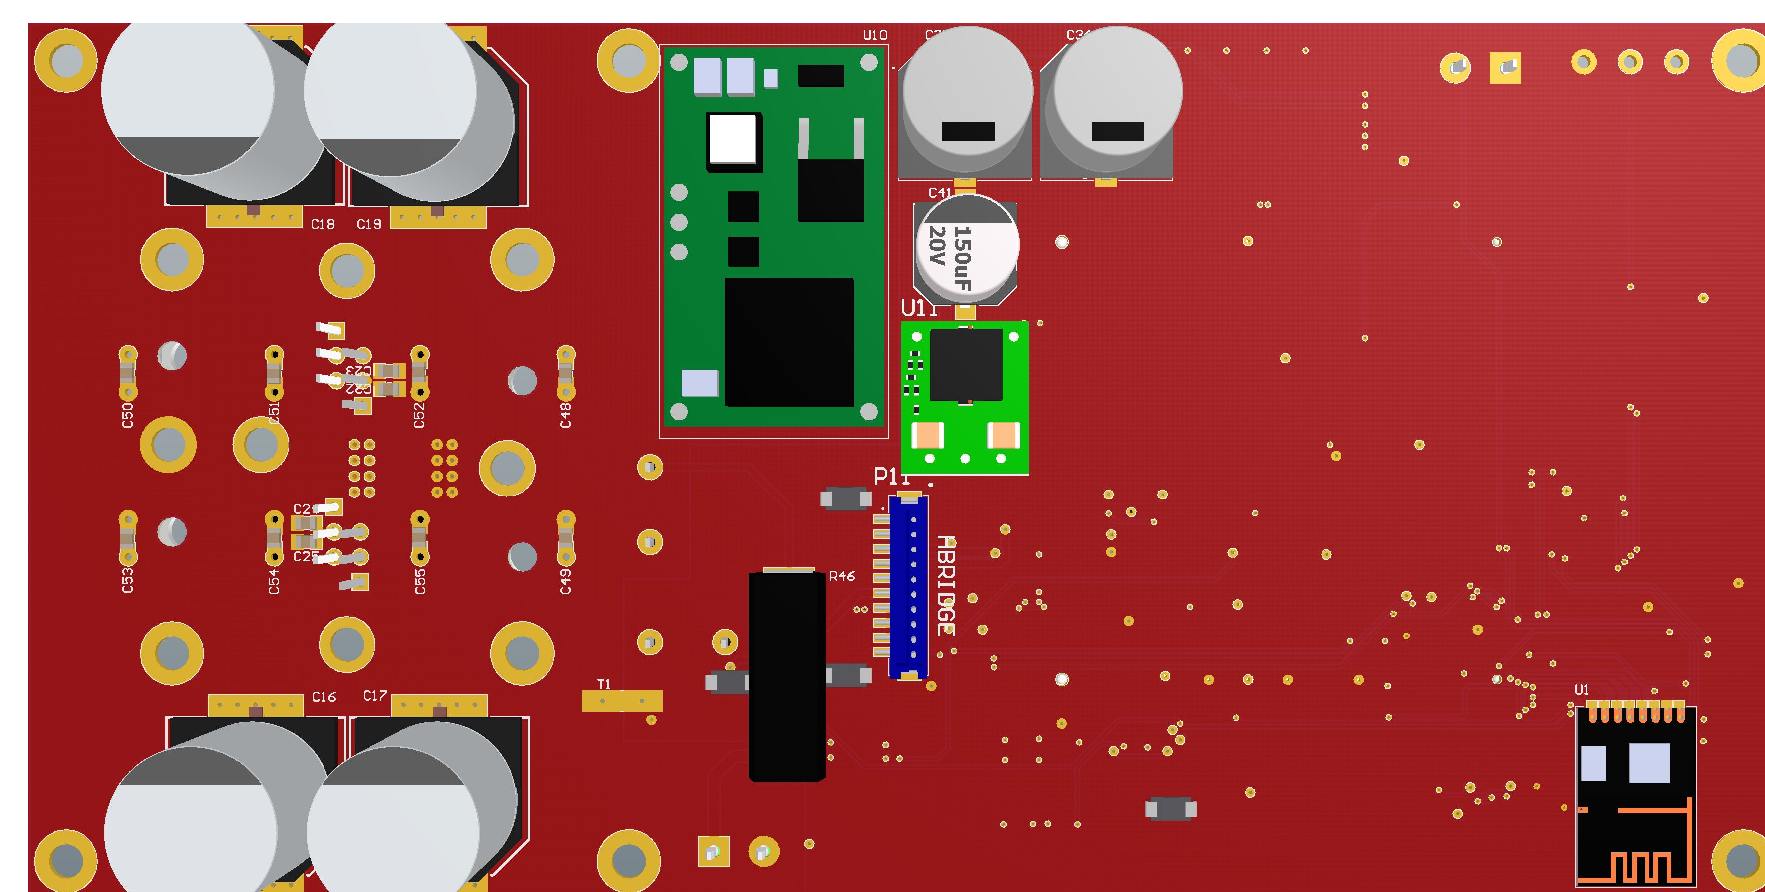
\includegraphics[width=0.8\textwidth,angle=180]{graphics/bottom_side_pcb}
	\caption{Bottom side PCB view of controller board.gull}
	\label{fig:botton_side_pcb_view}
	\end{subfigure}
	\caption{Top and bottom view of the controller board.}
	\label{fig:board_layout}
\end{figure}

\subsubsection{Copper Thickness}
Part of the board is designed to house the H-Bridge that drives the motor.
The H-bridge is designed to carry up to 80A, well above what can reasonably be carried at standard PCB copper thickness.
This section seeks to estimate the required copper thickness to allow for the design current.
Allowing a current through a conductor will produce a temperature rise due to the power dissipated in the conductor.
The current-carrying capacity (CCC) of a conductor is unlimited, so far as the current is not destructive due to the temperature rise permissable in the design.
Essentially, the acceptable temperature rise is limited by the maximum operating temperature of the PCB material.
This specification is known as the temperature index.
The PCB material most commonly used is FR-4 which has a temperature index of 130\degree \cite{fr4}.
At an ambient temperature of 20\degree this would imply a permissable conductor temperature rise of 110\degree.
In all practical situations, this is unreasonably high.
The material will discolor and degrade over time with the excessive heating and cooling of the board while also increasing the apparent ambient temperature of other components on the PCB, lowering the efficiency of the circuit.
\\~\\
In actual designs, a much more conservative temperature rise of 10\degree is often used, 15\degree is acceptable and 20\degree is considered high.
This was discussed with Jesper Nielsen, a technician at SDU who has experience in designing high power PCBs and it was decided to accept 15\degree increase. 
The actual temperature rise of a conductor is dependent on a great number of variables, among these are: conductor length, cross-sectional area, conductor material, PCB material, ambient temperature, convection, PCB layout (the amount of copper in the vicinity), etc.
\\~\\
Not all conductors carry the same current so different conductors have different thermal impacts on different locations on the PCB.
Clearly, it is difficult to accurately calculate the required copper thickness, however an estimate can be made.
In IPC-2221A \cite{ipc2221} data is presented to show the temperature rise resulting from allowing a current through a trace on a PCB on different trace widths.
This data was first published in \cite{conduct}, a progress report from the American National Bureau of Standards dating back to 1956.
Much has happened in PCB manufacturing since then. 
The original data does not take into account the possibility of multi-layered boards or many of the newer board materials.
In 2009 the new IPC-2152 \cite{ipc2152} was published and reevaluates the topic of current-carrying capacity.
This standard, however, is unavailable due to its high cost and the original charts are used instead.
A number of PCB trace width calculators exist online which extrapolate from the original data to give estimates of the required copper thickness and width.
One such calculator \cite{pcb_trace_calc} was used to determine the required copper thickness and width required in this project.
\\~\\
There are economic constraints in place for this project which requires the authors to be somewhat conservative with respect to how exotic a solution will be considered.
Most manufacturers support increasing the thickness of copper on a specific layer, allowing well above the 35$\mu$m standard copper thickness.
The manufacturer used in this project was chosen due to a comparatively low price on 4-layer boards with 70$\mu$m copper on outer layers and 52.5$\mu$m on internal layers.
On the power part of the board this results in a total of 122.5$\mu$m of copper for the 24V rail and power ground.
\\~\\
In order to simplify the design process, a distinction is made between three types of traces.
This distinction is based on the expected amount of current carried by that trace.
\begin{itemize}
	\item \textbf{Signal:} This is the type with the lowest expected current and is used throughout digital circuitry and low power analog signals.
	Signal traces are by far the most abundant on the circuit and due to the very low currents the trace width should be as small as possible.
	The manufacturer is capable of creating traces at 8 mil or higher at the desired copper thickness and as such the trace width for this type is 8 mil.
	\item \textbf{Power:} This type is generally used for supply rails.
	The trace width for this type is 20mil. Accepting 15\degree temperature increase will allow up to $\approx$1.5A of current.
	This is sufficient for supplying any of the IC's and other components connected to this trace type.
	\item \textbf{High Power:} This type is used exclusively for the 24V rail.
	The trace width for this type is 40mil. Accepting 15\degree temperature increase will allow up to $\approx$2.4A of current.
	Since the inrush current is limited to $\approx$0.14A this leaves plenty of headroom for creating the 2.5V, 3.3V, 5V and 12V rails.
\end{itemize}

\subsubsection{Copper Layout} % (fold)
\label{ssub:copper_layout}
The board can be split into two parts: a digital circuit and a power circuit.
As seen on figure \ref{fig:board_layout} the power circuitry is placed on the right third of the board while the digital circuitry occupies the remainder of the board.
The two parts have seperate ground planes in order to protect the digital circuitry from the high and sudden currents generated by the motor.
A ground plane, even though the resistance through it is low, will have a significant voltage drop across it if currents of sufficient magnitude are passed through it.
For the same reason it is desirable to keep the current path as short as possible on the power side of the board.
Figure \ref{fig:power_layout} depicts a 3D view and 2D view of the power part of the board.
As can be seen, the MOSFET's are bend such that a heatsink can be mounted on top.
The upper pair is the left half-bridge and the lower pair is the right half-bridge.
The outtake for the motor is positioned directly above and below the two half-bridges and a 3M bolt is mounted to allow for a robust connection.
A large pad is made where the bolt is mounted as close as possible to the MOSFET's to allow for unrestricted flow of current.
The pad between the motor outtakes is the connection from source of the low-side of the half-bridges to the shunt resistor used for current measurements.
Since all current must pass through the shunt resistor, it is crucial that the flow of current is as unrestricted as possible.
\\~\\
Main power is input through M3 bolts mounted in the three holes between the half-bridges.
Clearly, only two terminals are required but the three pads effectively divide the 24V rail into two parts, forcing any currents to flow around the pads.
Instead it was decided to use two input terminals for the 24V rails that are mechanically fixed at the bolts.
The ground plane is unrestricted and as such the current can flow freely and only one terminal is required.
None of the planes on the power side of the PCB can be interrupted by traces, as this would severely hinder the flow of current in that plane.
This means that it is necessary to add wires to carry the gate, return and shunt signals.
These wires are soldered directly to the MOSFET pins and connected to the digital side through a header on the bottom side of the board. 

\begin{figure}
	\centering
	\begin{subfigure}[b]{0.49\textwidth}
		\centering
		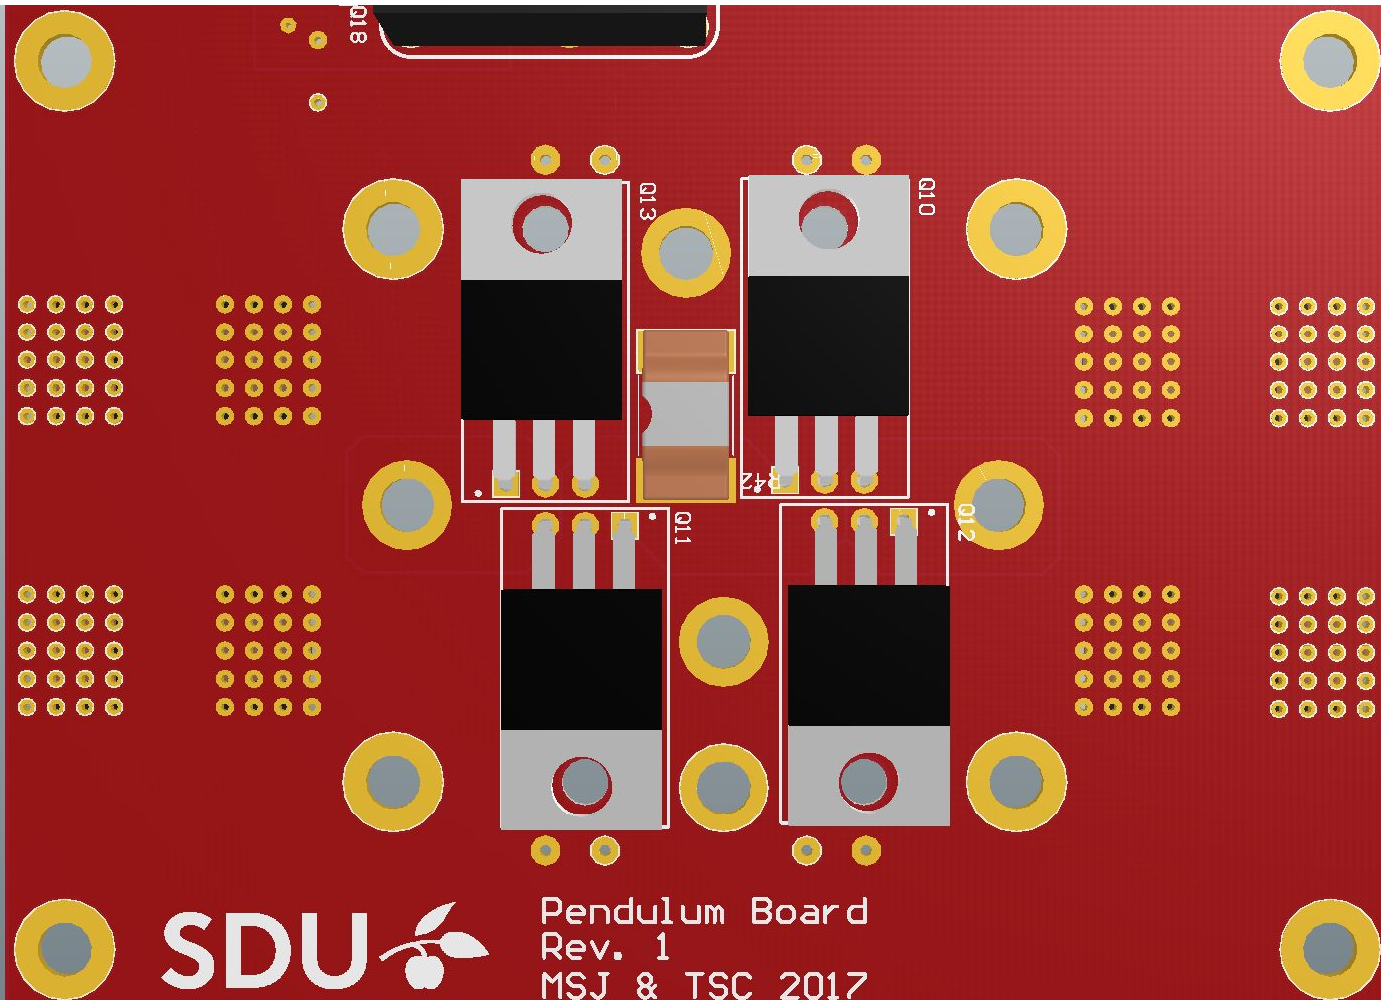
\includegraphics[angle=90,width=\linewidth]{graphics/power_layout_3}
		\caption{3D layout of the power part on the top layer}
		\label{sfig:power_layout_3}
	\end{subfigure}
	\begin{subfigure}[b]{0.49\textwidth} 
		\centering
		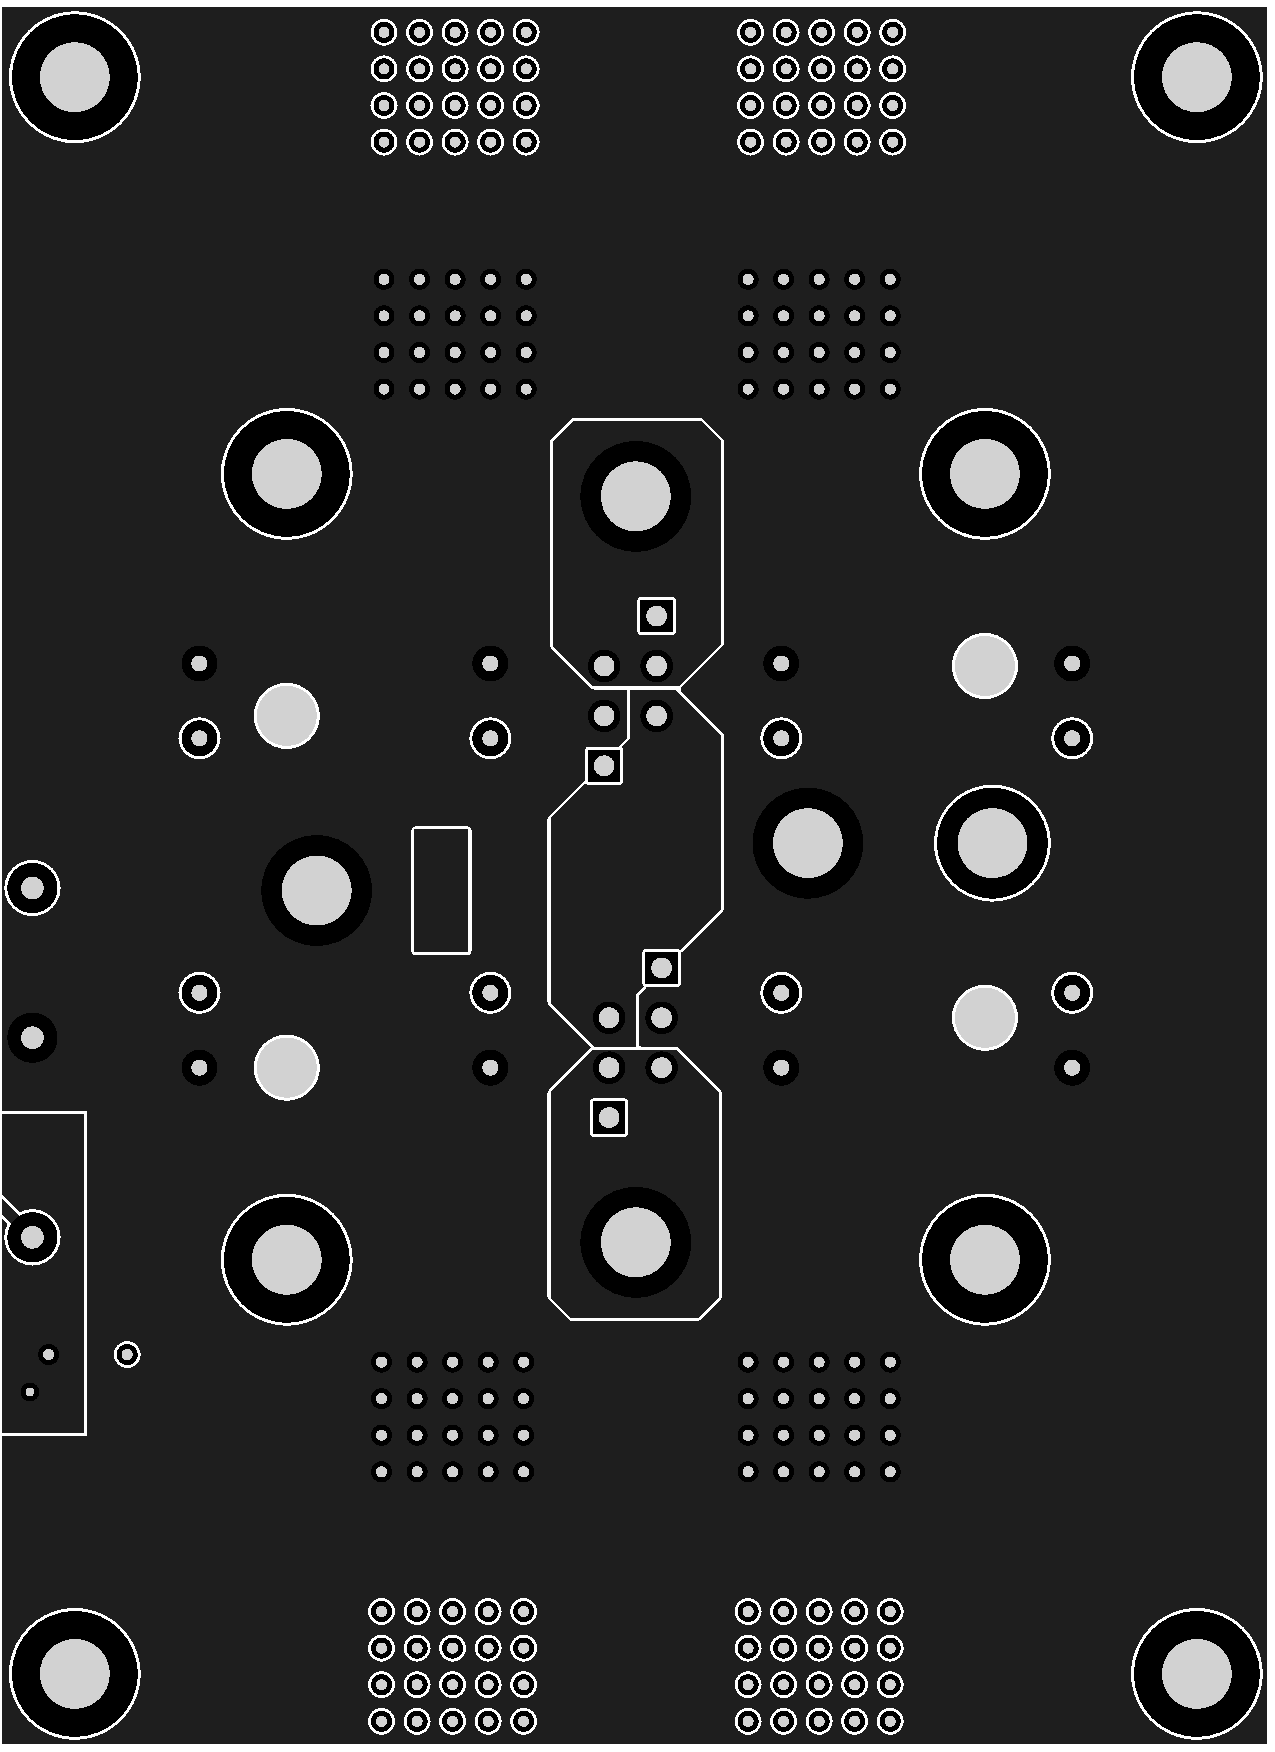
\includegraphics[width=\linewidth]{graphics/power_layout}
		\caption{Copper layout of the power part on the top layer.}
		\label{sfig:power_layout_2}
	\end{subfigure}
	\caption{Power layout on the controller board.}
	\label{fig:power_layout}
\end{figure}
~\\
As mentioned previously it was chosen to use a 4-layer board.
This was done for two reasons: It gives more copper for the main power rails on the power side of the board and it allows more space for routing signals on the digital part of the board.
While the component density is not very high, the number of signals routed to headers does impose some difficulties routing on just two layers.
On the digital side, a pour is made on each layer to fill the unused part of the layer with copper.
Going from top to bottom the layers are as such: ground, ground, 5V, ground.
The internal ground layer is uninterrupted, except for vias, to provide a solid ground layer.
The 5V layer means that any components requiring 5V need only a via to access it, making routing simpler.
This layer is also used for routing when routing through the top and bottom layers is infeasible.

% paragraph copper_layout (end)
% paragraph component_case_selection_and_placement (end)
% section board_design (end) 


